% \section{System-Level Analysis} \label{sec:results}
\section{Baseline I/O Performance} \label{sec:results}


We first establish the baseline performance variation of each benchmark on each system tested.
% Such variation in peak file system performance caused by different I/O access patterns is well documented~\cite{Lofstead2010,Uselton2010,Xie2012}.
Because variation in peak I/O performance is known to be caused by different I/O access patterns~\cite{Lofstead2010,Uselton2010,Xie2012}, 
% To focus solely on the variation caused by factors \emph{extrinsic} to each application,
we define the \emph{fraction of peak performance} as the performance of a job divided by the maximum performance observed for all jobs \emph{of the same I/O motif} as listed in Table \ref{tab:bench-config} and whether the job did reads or writes.
For example, the fraction peak performance for a HACC write test is only normalized to the maximum performance of all other HACC write tests on the same file system.

The distribution of fraction peak performance, shown in Figure~\ref{fig:perf-summary-boxplots-motif}, reveals that the degree of performance variation \emph{within} each application varies with each file system.
For example, the HACC write workload is susceptible to a long tail of performance degradation on mira-fs1 despite that file system's overall lower variation as evidenced by the distance between all I/O motifs' whiskers relative to the Edison file systems.
% Similarly, all Edison file systems show a long tail of performance loss for the IOR/shared file read workload.
Edison's scratch3 also demonstrates very broad performance variation for the VPIC write workload, contrasting with the relatively narrow performance variation of this application on other systems.

\begin{figure}[t]
    \centering
    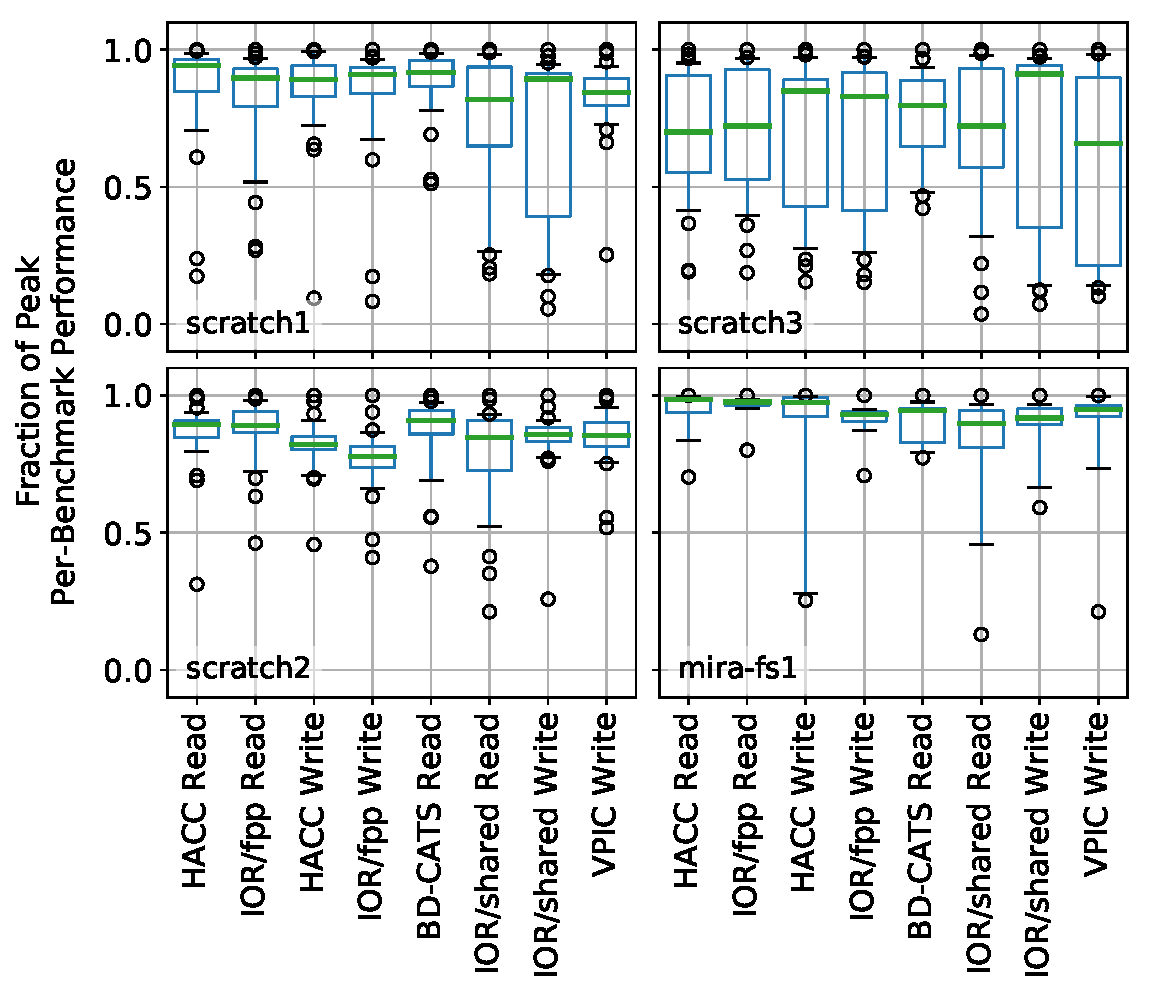
\includegraphics[width=1.0\columnwidth]{figs/perf-boxplots.pdf}
    \caption{I/O performance for all file systems tested grouped by test
    applications and read/write mode.  Whiskers represent the 5th and 95th
    percentiles.}
    \label{fig:perf-summary-boxplots-motif}
\vspace{-.2in}
\end{figure}

We can conclude from this that performance variability is the result of factors intrinsic to the application \emph{and} factors intrinsic to the file system;
different I/O motifs result in different levels of performance \emph{and} variability.
Furthermore, these behaviors are not a function of the parallel file system architecture either; all Edison file systems are Lustre-based, yet Figure~\ref{fig:perf-summary-boxplots-motif} shows a marked difference in variability between scratch1/scratch2 and scratch3.
Thus, these differences in performance variation must be a result of their different hardware configurations (discussed in Section \ref{sec:platforms}), their specific user workloads, or a combination of both.
This finding highlights the importance of examining multiple sources of I/O characterization data (e.g., application-level and server-side) in concert to develop a full understanding of I/O performance.

%%%%%%%%%%%%%%%%%%%%%%%%%%%%%%%%%%%%%%%%%%%%%%%%%%%%%%%%%%%%%%%%%%%%%%%%%%%%%%%%
% \subsection{Combined Application/Server Metrics} \label{sec:results/combining}
%%%%%%%%%%%%%%%%%%%%%%%%%%%%%%%%%%%%%%%%%%%%%%%%%%%%%%%%%%%%%%%%%%%%%%%%%%%%%%%%

% \begin{figure}[t]
%     \centering
%     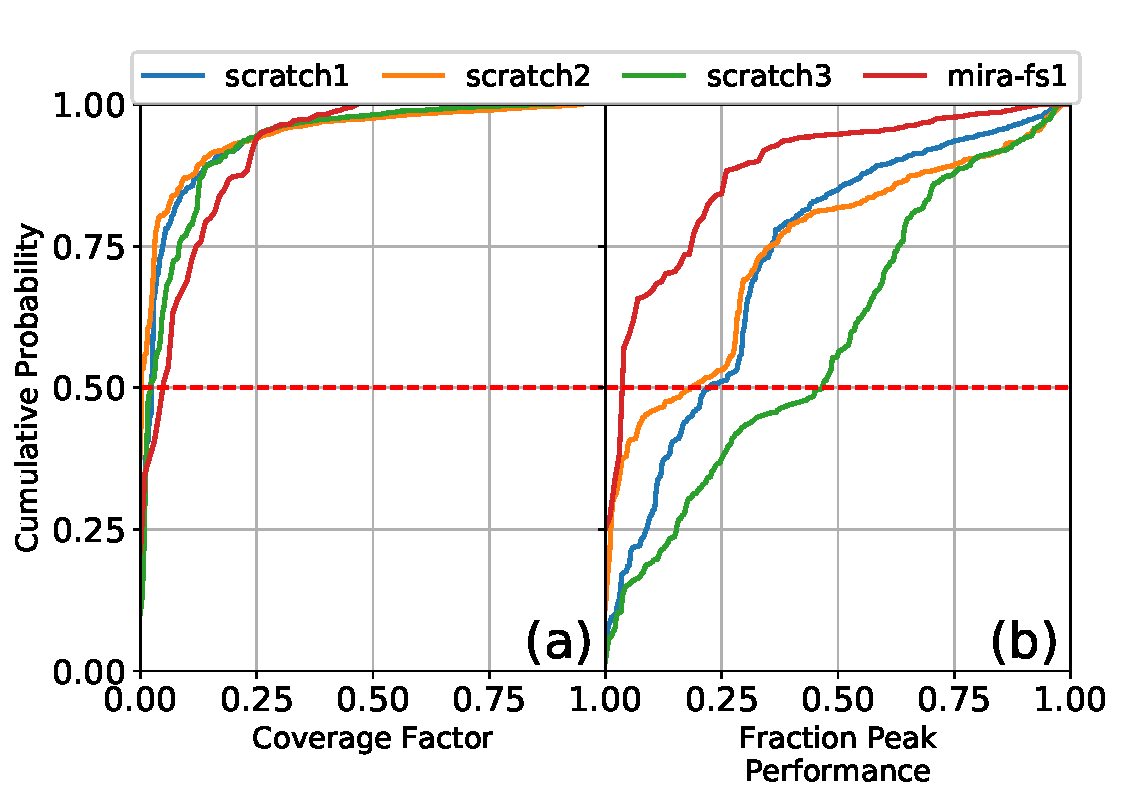
\includegraphics[width=\columnwidth]{figs/cdf-both.pdf}
%     \caption{Cumulative distribution function of the coverage factor (a) and the    performance relative to the maximum throughput observed across each file system (b).
%     The line demarcating 50\% probability corresponds to coverage factors of 0.88, 0.87, 0.84, and 0.94 and peak performance fractions of 0.89, 0.86, 0.78, and 0.95 on Edison scratch1-scratch3 and Mira, respectively.}
%     \label{fig:cdfs}
% \vspace{-.2in}
% \end{figure}

%The distribution of coverage factors across all experiments run are shown in Figure~\ref{fig:cdfs}a which reveals that the majority of tests ($> 75\%$ on Edison and $> 80\%$ on Mira) have high coverage factors ($\mathit{CF} > 0.80$).
%This is consistent with the observation that I/O occurs in bursts~\cite{Carns2011,Liu2016}, and the probability of two bursts coinciding and causing contention for bandwidth (thereby reducing $\mathit{CF}$) is relatively low.
%In particular, Mira's $\mathit{CF}$ distribution is so narrow that over 50\% of tests effectively ran without bandwidth contention; $\mathit{CF} >= 0.99$ corresponds to the 40th percentile on that system.

% Across all benchmark runs, over 75\% (Edison) and 80\% (Mira) of the measurements analyzed had high coverage factors ($\mathit{CF} > 0.80$).
% This is consistent with the observation that I/O occurs in bursts~\cite{Carns2011,Liu2016}, and the probability of two bursts coinciding and causing contention for bandwidth (thereby reducing $\mathit{CF}$) is relatively low.
% In particular, Mira's $\mathit{CF}$ distribution is so narrow that over 50\% of tests effectively ran without bandwidth contention; $\mathit{CF} >= 0.99$ corresponded to the 40th percentile on that system.
% 
% Despite this low incidence of overlapping bursts, the distribution of performance relative to the peak observed bandwidth for each application such as shown in Figure~\ref{fig:perf-summary-boxplots-motif} is more broadly distributed.
% Edison's scratch3 exemplifies this; 26\% of jobs on that file system got less than half of the peak performance (fraction peak performance $< 0.50$) despite only 5\% of jobs showing $\mathit{CF} < 0.50$.  This indicates that the coverage factor (and therefore server-side I/O bandwidth) is not the only contributor to I/O performance degradation.
% This finding is consistent with previous work that found Lustre file system performance to be constrained by both bandwidth \emph{and} I/O operation (IOP) rate~\cite{Uselton2013}.

% \begin{figure}[t]
%     \centering
%     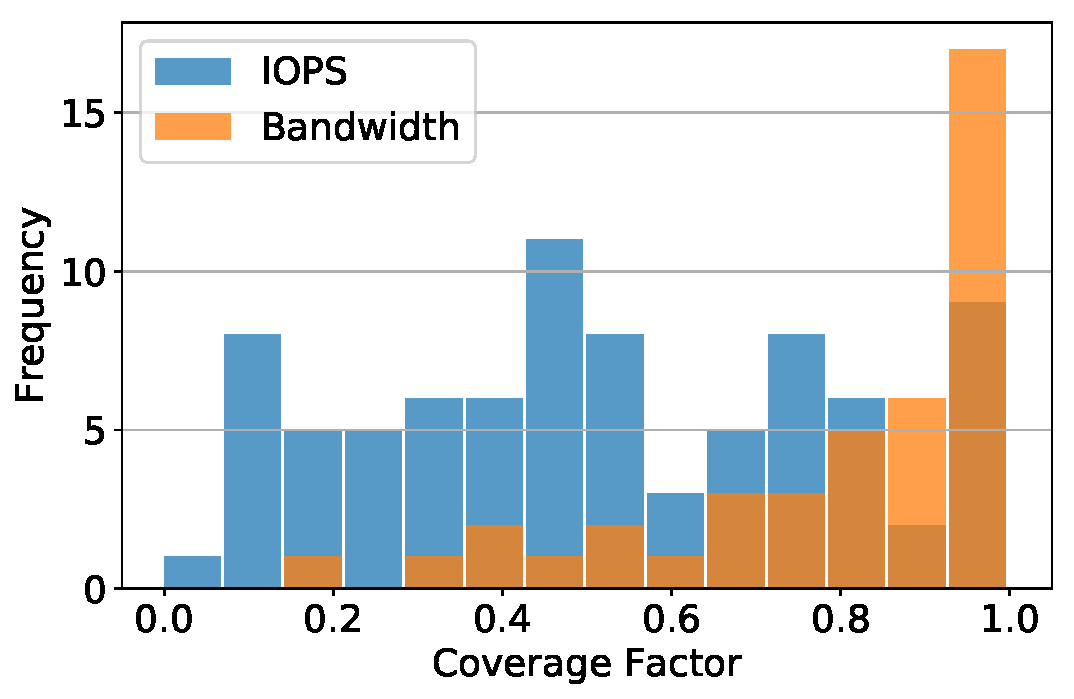
\includegraphics[width=\columnwidth]{figs/hist-cf-bw-and-ops.pdf}
%     \caption{Distribution of the coverage factor for both bandwidth ($\textit{CF}_{\textup{bandwidth}}$) and read/write operations ($\textit{CF}_{\textup{iops}}$) for Mira.
%     }
%     \label{fig:hist-cf-mira}
% \vspace{-.2in}
% \end{figure}
% 
% We can generalize this notion of the coverage factor to any metric for which we can distinguish the contribution of an individual job from the global system-level measurement.
% However, these alternative coverage factor metrics are not likely to correlate well with performance unless the job of interest is making a meaningful contribution to the system-wide load.
% For example, the coverage factor for IOPs can be expressed as the fraction of read and write operations extracted from a job's Darshan log to the total read and write operations logged by ggiostat.  The distribution of this $\textit{CF}_\textit{IOPs}$ metric is shown alongside the bandwidth coverage factor, $\textit{CF}_\textit{BW}$, in  Figure \ref{fig:hist-cf-mira}.
% This figure suggests that the TOKIO-ABC tests likely do not contribute a significant IOPs load Mira;
% the relatively flat distribution of $\textit{CF}_\textit{IOPs}$ is likely a reflection of the background IOPs load which is not significantly perturbed when TOKIO-ABC jobs are running. \todo{is there is a clearer way to state the previous sentence?}
% 

%%%%%%%%%%%%%%%%%%%%%%%%%%%%%%%%%%%%%%%%%%%%%%%%%%%%%%%%%%%%%%%%%%%%%%%%%%%%%%%%
% \subsection{Correlating Performance Metrics} \label{sec:results/correlating}
%%%%%%%%%%%%%%%%%%%%%%%%%%%%%%%%%%%%%%%%%%%%%%%%%%%%%%%%%%%%%%%%%%%%%%%%%%%%%%%%

% Given the observation that bandwidth contention is not the sole source of performance variability, 
% % Although bandwidth is the most intuitive initial metric for application and server correlation,  
% %Our choice to define our correlation parameter according to application performance and server-side bandwidth and IOPs was motivated by a broad body of literature and an intuitive assumption that competition for bandwidth and IOPs affect performance the most dramatically.
% %the TOKIO framework is generalized to draw data from any resource that can be indexed on a per-job or time series basis.
% %Thus,
% % we can 
% we then establish correlations between job I/O performance and other metrics to identify which components in the I/O subsystem are the most likely causes of poor I/O performance.
% To this end, we calculated the Pearson correlation coefficient between each job's fraction of peak performance (defined in \ref{sec:results/overview}) with the range of metrics described in Section \ref{sec:methods}.
% While many of these metrics are not expected to be normally distributed~\cite{Kim2010}, Pearson correlation coefficients are applied here to compare the directions and relative strengths of the relationships between each metric we analyzed.
% As such, this correlation coefficient is a suitable qualitative indicator of general trends and confidences despite the unknown distribution of each underlying component's metrics.
% A summary of some of the most notable correlations (or lack thereof) are presented in Figure \ref{fig:correlation-table} and highlight several interesting findings:
% 
% \begin{figure}[t]
%     \centering
%     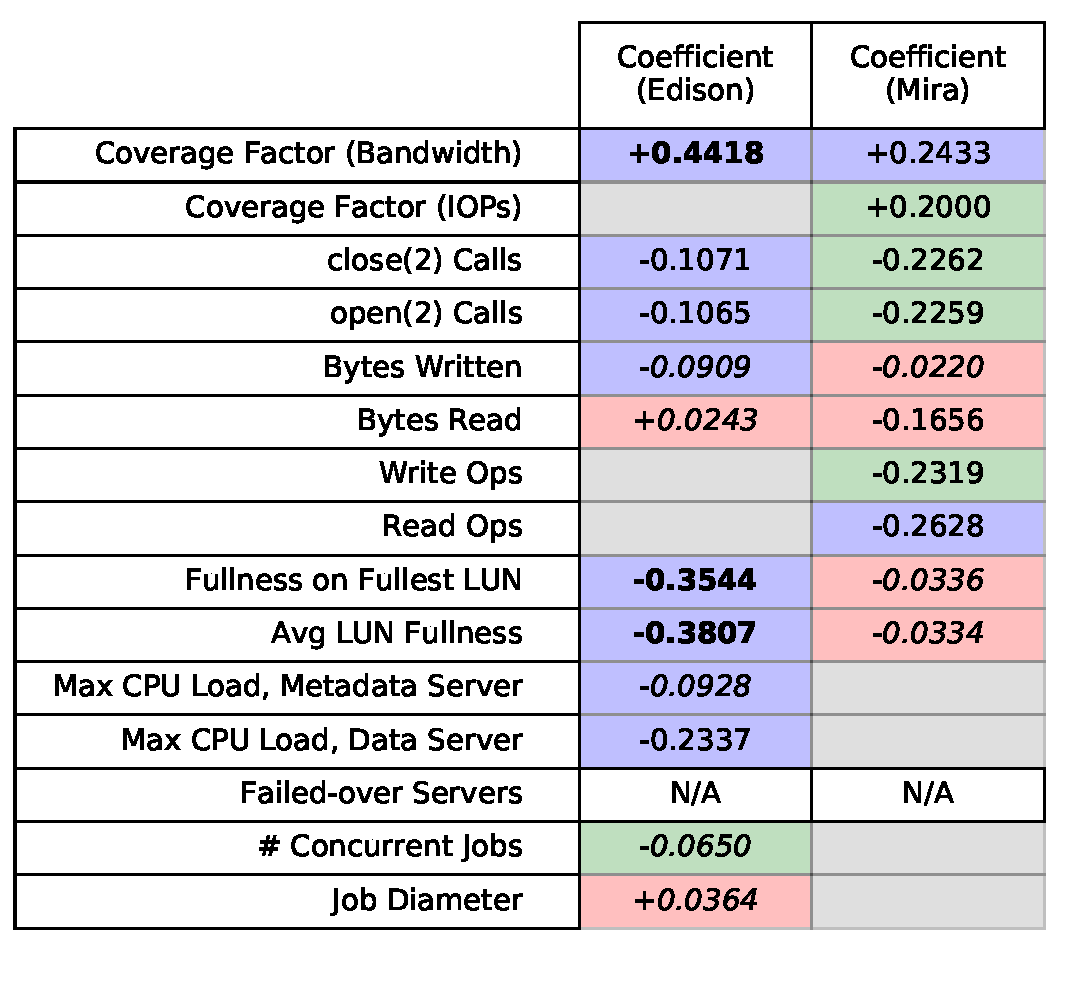
\includegraphics[width=\columnwidth]{figs/correlation_table.pdf}
%     \caption{Correlation coefficients between fraction of peak performance measured for each I/O motif and a variety of server-side measurements and metrics.
%     Box color indicates confidence; correlations with p-values $< 0.01$ are blue; p-values $< 0.05$ are green, and p-values $>= 0.05$ are red (and signify lack of correlation).
%     Similarly, \textbf{bolded} values signify moderate correlation ($|r| > 0.30$), and \textit{italicized} values signify weak correlation ($|r| < 0.10$).
%     The "\% Servers Failed Over" metric is not applicable because no
%     changes in server failover state were
%     observed during this study.
%     }
%     \label{fig:correlation-table}
% \vspace{-.2in}
% \end{figure}
% 
% \begin{itemize}[leftmargin=*]
% 
% \item CFs correlate with performance on all file systems, indicating that contending for file system I/O is a moderate contributor to performance loss.
% This correlation is less strong on Mira because the absolute performance of our tests on Mira were limited by the bandwidth of the I/O nodes allocated, leaving bandwidth headroom on the NSD servers for other jobs.
% Mira's file system also demonstrated moderate sensitivity to contention for
% IOPs confirming the generalizability of the conclusions of Uselton and Wright~\cite{Uselton2013} based on Lustre performance.
% %Lustre IOPs were not collected for this study, so no comparison can be made to Edison.
% 
% \item Mira's performance correlates negatively with higher rates of \texttt{open(2)}/\texttt{close(2)} calls than Lustre.
% This is reasonable given that Mira's file system serves metadata from the same physical servers as data.
% By comparison, Edison's file systems each have their own discrete metadata servers that are specifically designed to decouple bulk data transfer performance from metadata operations.
% 
% \item File system fullness has markedly different behavior on Edison relative to Mira.
% While Mira's performance is uncorrelated with device capacity, Edison performance degrades as free space on OSTs is depleted.
% This type of behavior is a known characteristic of the Lustre file system and has been observed on deployments at other HPC centers~\cite{oral2014best}.
% 
% \item Contrary to our expectation, I/O performance shows minimal correlation with the number of other jobs running concurrently.
% The lack of correlation is consistent with our finding that I/O remains highly bursty; a large number of small jobs are highly unlikely to burst simultaneously, and each small job is not individually capable of significantly impacting our tests' coverage factors.
% 
% % \item Similarly, the job diameter (a measurement of how spread out a job is across the compute fabric) has no discernible correlation with I/O performance on Edison.
% % Since the low-diameter dragonfly topology of Edison is designed
% % to reduce the performance impact of job topology, this is consistent with
% % expectation.  Job diameter is not shown for Mira because it utilizes a dense
% % torus partition for each job.
% 
% \end{itemize}
% 
% %We collected additional system-specific measurements that did not correlate significantly to performance.
% %However this correlation analysis was not intended to be exhaustive, and the correlations and p-values for the Edison system are likely diminished by the fact that data for all three Edison file systems were combined for this analysis.

%%%%%%%%%%%%%%%%%%%%%%%%%%%%%%%%%%%%%%%%%%%%%%%%%%%%%%%%%%%%%%%%%%%%%%%%%%%%%%%%
\section{Integrated Analysis} \label{sec:results/umami}
%%%%%%%%%%%%%%%%%%%%%%%%%%%%%%%%%%%%%%%%%%%%%%%%%%%%%%%%%%%%%%%%%%%%%%%%%%%%%%%%

With an understanding of the baseline performance variation on each system and I/O motif tested, we can then combine the application performance data derived from Darshan with server-side load data derived from LMT/ggiostat to
better understand how performance variation is caused by factors extrinsic to the application.
I/O bandwidth contention from other jobs is an intuitive source in I/O performance variation, so we define the \emph{coverage factor} ($\mathit{CF}$) of a job $j$ to quantify the effects of such competing I/O traffic:

\begin{equation} \label{eq:cf}
    \mathit{CF}(j) = \frac{N_{\textup{bytes}}^{\textup{Darshan}}(j)}
    {\sum_{t,s}^{\textup{time,servers}}
    \left [ N_{\textup{bytes}}^{\textup{LMT,ggiostat}}(t,s) \right ] }
\end{equation}
%
where $N_{\textup{bytes}}^{\textup{Darshan}}$ are the bytes read and written by job $j$ from to its Darshan log, and $N_{\textup{bytes}}^{\textup{LMT,ggiostat}}$ are the bytes read and written to a parallel file system server $s$ during a 5-second time interval $t$.
The time interval over which the job ran ($\mathit{time}$) and the servers to which the job wrote ($\mathit{servers}$) are both taken from the job's Darshan log~\cite{snyder2016modular}.
% It should be noted that we can generalize this notion of the coverage factor to any metric for which we can distinguish the contribution of an individual job from the global system-level measurement, but for brevity in this work we focus our analysis on bandwidth coverage factor.

This CF is a direct reflection of how much I/O traffic a job competed against in the underlying file systems.
When $\mathit{CF} = 1.0$, all of the server-side I/O can be attributed to job $j$, while $\mathit{CF} = 0.5$ indicates that only half of the server-side I/O is attributable to job $j$ while the other half is from other sources.
%In practice, $\mathit{CF}$ can be slightly greater than $1.0$ as a result of two conditions:
%a) when the storage system traffic monitoring (LMT/ggiostat) does not capture data from all servers during a polling interval, or
%b) when clock skew between the compute nodes and the file system servers causes the Darshan log and LMT/ggiostat to have an inconsistent understanding of when I/O happened.
%In this study, such noise never resulted in $\mathit{CF} > 1.2$.
%%%% GKL: The ratio of CF > 1.2 to all CF measurements is very high on Mira; 96 of the 214 measurements provided by Shane were dropped due to this filter criterion

This CF metric, along with the system health, job scheduling, and job topology data then allow us to contextualize performance anomalies and describe where on the spectrum of normalcy a job's I/O performance fell relative to jobs with similar motifs, and it can point to the metrics that are most likely culprits for investigation based on historic correlation.

\begin{figure}[t]
    \centering
    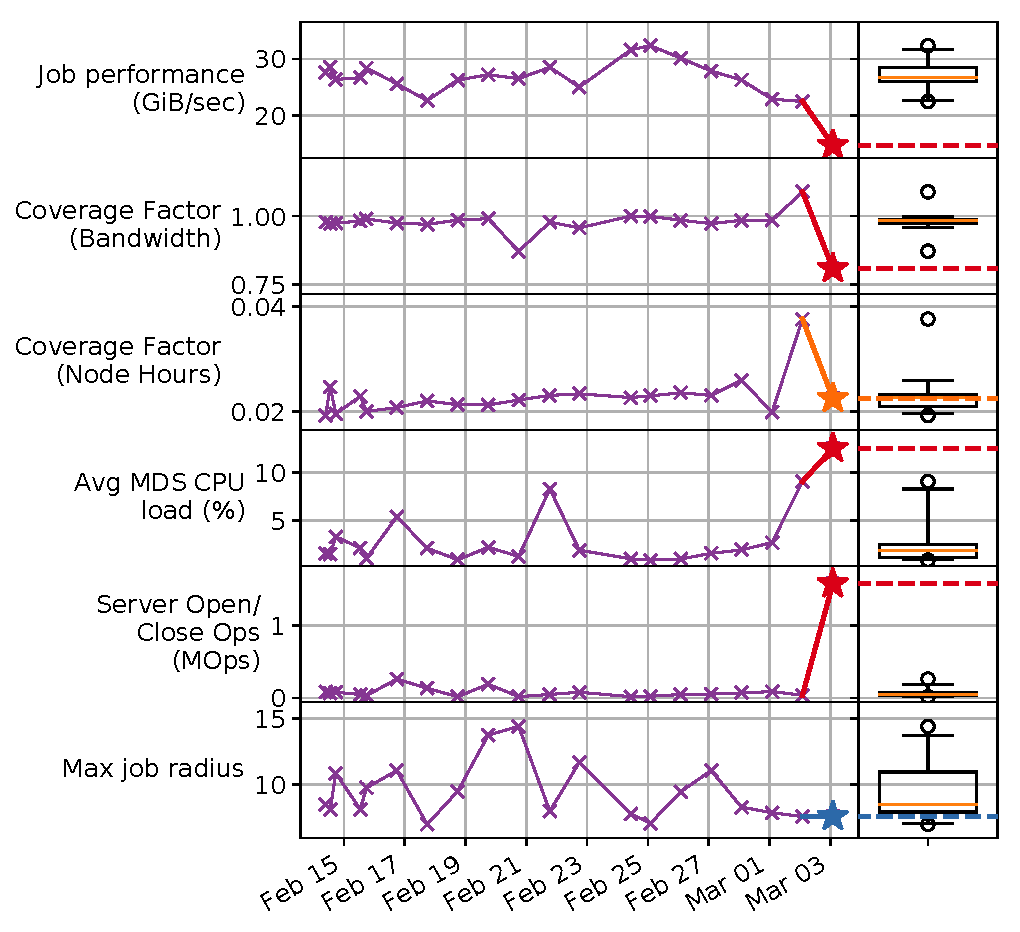
\includegraphics[width=1.0\columnwidth]{figs/umami-scratch2-hacc-write.pdf}
    \caption{UMAMI demonstrating the \emph{file system climate} of HACC write workloads on the Edison scratch2 file system compared to a most recent run, which showed highly unusual \emph{file system weather}.
    The left panes show the measurements from previous runs of the same motif, and the box plots in the right panes summarize the distribution of these metrics.
    The star denotes the metrics for the job of interest and is colored according to the quartile in which it falls (red being the worst quartile and blue the best).
    Box plot whiskers extend to the 5th and 95th percentiles, with outliers being denoted as circles.}
    \label{fig:umami-scratch2-hacc-write}
\vspace{-.2in}
\end{figure}

To concisely visualize all of this information, we present a Unified Measurements And Metrics Interface (UMAMI) diagram as a tool to quickly determine how a job of interest's performance compares to similar I/O workloads in the past.
UMAMI, demonstrated in Figure \ref{fig:umami-scratch2-hacc-write}, presents historic measurements (the I/O climate) and summarizes each metric's distribution in an accompanying box plot.
These time series plots terminate with the metrics for the job of interest and define the I/O weather at the time that job ran.
By overlaying this weather on the climate (dashed lines in the box plots), UMAMI provides a quick view of how each metric compared to the statistical distribution of past weather conditions.
With this juxtaposition of a file system's weather and its overall climate, a user can differentiate between a long-term performance problem and a statistically rare event.% analogous to an extreme weather event.

% In the following sections, we illustrate how UMAMI can be applied to the problem of diagnosing poor performance of individual jobs in three case studies.

\subsection{Case Study: I/O Contention}

The specific UMAMI example shown in Figure \ref{fig:umami-scratch2-hacc-write} represents a HACC write test which took place on March 3.
Per the "Job performance" measurement and its value relative to previous instances of this type of job, this job's performance is statistically abnormal.
This poor performance was accompanied by an unusually low coverage factor and high metadata load, and these unfavorable conditions are highlighted as red dashed lines in the box plots that denote their place in the least-favorable quartile of past measurements.
The metrics corresponding to blue dashed lines fell into the most favorable quartile for this problematic job, but they were also not found to correlate with performance.
Thus, we can attribute this HACC job's poor performance to I/O loads extrinsic to this job which competed for both bandwidth and metadata operation rates.

\subsection{Case Study: Metadata Load}

Figure \ref{fig:umami-mira-fs1-vpic-write} represents a VPIC write workload
that showed poor performance on Mira.
Its coverage factor is within normal parameters (orange lines in the box plots denote a value in the second quartile) indicating low bandwidth contention.
Although the IOPS coverage factor is also low, previous conditions have been worse despite a lack of dramatic performance loss (e.g., on March 7).
The only metric that shows a unique, undesirable value is the number of \texttt{readdir(3)} operations handled by the file system.
This is indicative of an expansive file system traversal that was being performed at the same time as the job execution.
% The \emph{readdir(3)} metric was demonstrated to correlate moderately negatively with performance in Figure \ref{fig:correlation-table}.

\begin{figure}[t]
    \centering
    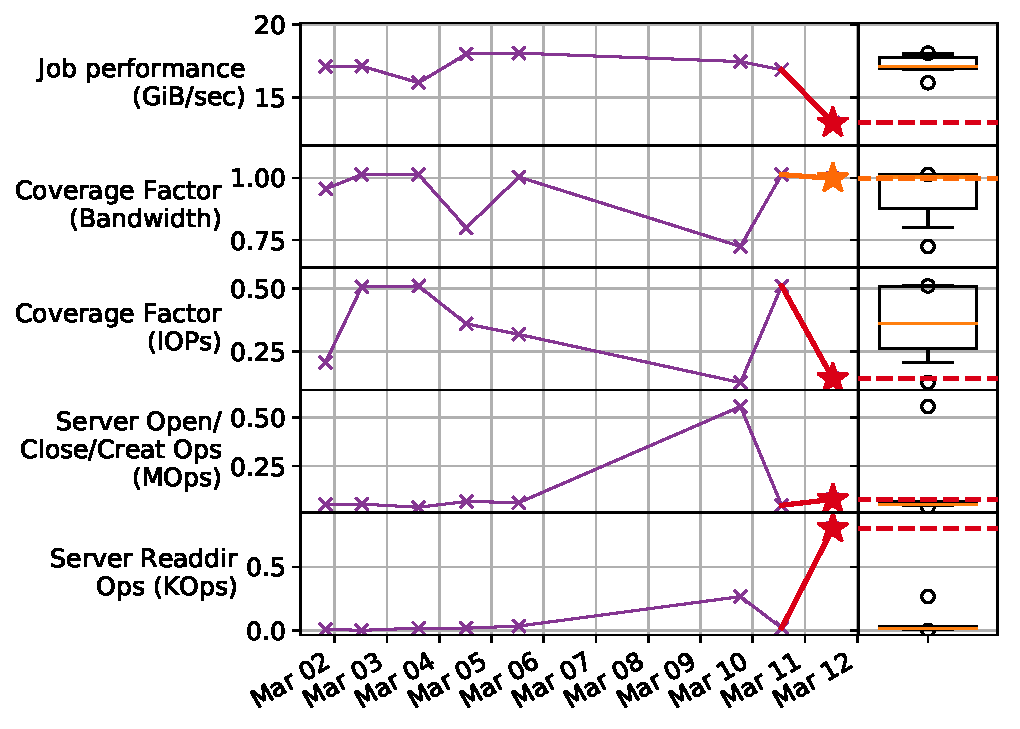
\includegraphics[width=1.0\columnwidth]{figs/umami-mira-fs1-vpic-write.pdf}
    \caption{UMAMI demonstrating the climate surrounding VPIC-IO write workloads on Mira compared to a most recent run, which showed highly unusual weather in the form of an excess of \texttt{readdir(3)} calls.
%   Significance of each pane and its contents are the same as explained in Figure \ref{fig:umami-scratch2-hacc-write}.
    }
    \label{fig:umami-mira-fs1-vpic-write}
\vspace{-.2in}
\end{figure}

%%%%%%%%%%%%%%%%%%%%%%%%%%%%%%%%%%%%%%%%%%%%%%%%%%%%%%%%%%%%%%%%%%%%%%%%%%%%%%%%
\subsection{Case Study: Storage Capacity}
%%%%%%%%%%%%%%%%%%%%%%%%%%%%%%%%%%%%%%%%%%%%%%%%%%%%%%%%%%%%%%%%%%%%%%%%%%%%%%%%

This holistic approach is also able to identify longer-term performance degradation.
Figure \ref{fig:umami-scratch3-hacc-write-long-term} shows the UMAMI view of such an event on Edison's scratch3 file system where coverage factors were not unusual despite an ongoing $2\times$ slowdown over the normal 50 GiB/sec.
The magnitude of performance loss followed the highest CPU load observed across all of the Lustre OSSes almost exactly, and this period coincided also with the scratch3 file system reaching critical levels of fullness.
Although such correlations cannot define causative relationships, these conditions indicated a relationship between critically full storage devices and CPU load (e.g., an increasing cost of scavenging empty blocks) that impacts application performance.
Incidentally, this behavior is consistent with known performance losses that result from Lustre OSTs filling~\cite{oral2014best}.
 
\begin{figure}[t]
    \centering
    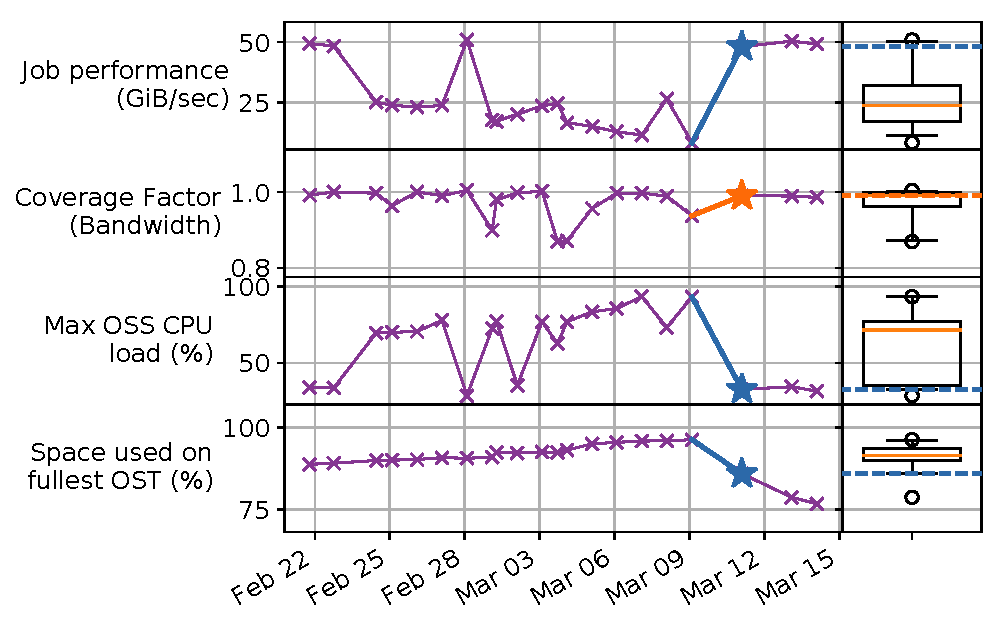
\includegraphics[width=1.0\columnwidth]{figs/umami-scratch3-hacc-write-long-term.pdf}
    \caption{UMAMI of HACC write performance on Edison's scratch3 file system showing a longer-term period of performance degradation that was associated with unusually high OSS CPU load.
%   Significance of each pane and its contents are the same as explained in Figure \ref{fig:umami-scratch2-hacc-write}.
    }
    \label{fig:umami-scratch3-hacc-write-long-term}
\vspace{-.2in}
\end{figure}
